\chapter[Current Progress]{Current Progress}

\section{Background}

Work started on the \gls{cita} on gls{chip} project in early 2015. Since then, we have developed interactive homework questions as well as tools that can track and analyze student progress. This parallel development of problems and analysis tools will ensure that we can continuously improve the system over many semesters in a structured way. It also ensures that we can react to change in an efficient manner.

\section{Development of CITA}

In order to create a consistent and effective system, I have divided the structure of \gls{cita} up into three main parts - Shallow CITA, Immersive CITA, and Postscripts. A single homework problem usually has all three of these pieces, but might omit one if it is not appropriate for the analysis. None of these individual pieces are functional on their own - it is only when they are combined in the proper way does the interactive analysis become useful.

\subsection{Shallow CITA}

Shallow CITA anticipates and corrects simple mistakes in student answers. This might include unit errors, misreading the question, or sign errors. It is intended to help students correct simple errors that would otherwise lose them easy points. It is useful because it highlights misconceptions that students have about physics concepts. In other words, Shallow CITA is meant to catch all of the ``low hanging fruit'' - the easy problems that can be solved with minimal trouble.

Shallow CITA does not transition the user to a new interface. Therefore, it does not have enough space to set up a new model or derive new equations. Instead, it simply displays a short message (one paragraph or less) so that the user can make minor corrections to his or her analysis and continue with the remainder of the homework assignment.

\subsection{Immersive CITA}

Immersive CITA gives a step-by-step walkthrough of the specific homework problem. Unlike other scaffolding systems, it does not simply give an algorithmic list of steps. Instead, students have to answer questions and work through the example in real time. Additionally, problems with multiple solution paths will have a branching structure by which students can make progress.

Immersive CITA is not supposed to be an artificial intelligence. Instead, it provides the structure that students need to think about a problem. It encourages discussion over algorithms. Thus, immersive CITA guides students through problems so that they have the background knowledge needed to participate in discussions.

\subsubsection{Branching Structures}

\pagebreak

\begin{table}[!ht]
  \centering
  \begin{tabular}{|p{2.7cm}|p{5.4cm}|p{4.6cm}|}
    \hline
    \textbf{Structure} & \textbf{Description} & \textbf{Examples}\\
	\hline
	No Structure & Some problems do not require the sophistication of a branching structure due to their simple nature. Other problems are meant to assess student performance, so a branching structure would skew results.
 & Weekly Reading Quiz Problems, Diagnostic Problems, Practice Test Problems\\
	\hline
	Single Hint & This structure is useful for problems that are relatively easy to do after students realize one key concept. Once students realize the ``trick'' the remaining analysis is straightforward. & Drawing a Good Diagram Before Using Superposition, Rayleigh Criteria, Geometric Optics\\
	\hline
	Linear & These are problems that have one preferred solution that is taught in an introductory physics student. We try to avoid using this structure as much as possible. However, when it is used, checkbox and numerical questions point out common misconceptions. & Thin Film Interference, Wave Equation\\
	\hline
	Recombination & Students realize that two seemingly different paths of logic are related. This structure is great for derivations because it shows students that there is more than one way to get from point A to point B.
 & Coulomb’s Law vs. Gauss’s Law for Continuous Charge Distributions\\
	\hline
	Tree & Each step in the analysis leads to new, unique steps. These might branch out into further unique steps. Depending on the analysis, students may get seemingly different answers. & Electric Circuits, Using Different Coordinate Systems in Some Problem\\
	\hline
	Dead End & Students analyze a problem in a reasonable way, learning later why their thought process was flawed. This structure lets students make mistakes - one of the most important parts of learning. & Integrating With Respect to Certain Variables Rather Than Others, Right Hand Rules\\
	\hline
  \end{tabular}
  \caption{Branching Structures}
  \label{tab:structures}
\end{table}

See the table for statistics on the questions. Notice how we have increased the number of linear and branching questions from spring to summer. Linear questions include those with only one single hint or a single, step-by-step path. Branching questions are those that involve tree, recombination, and dead end structures.

\begin{figure}[!htb]
	\centering
	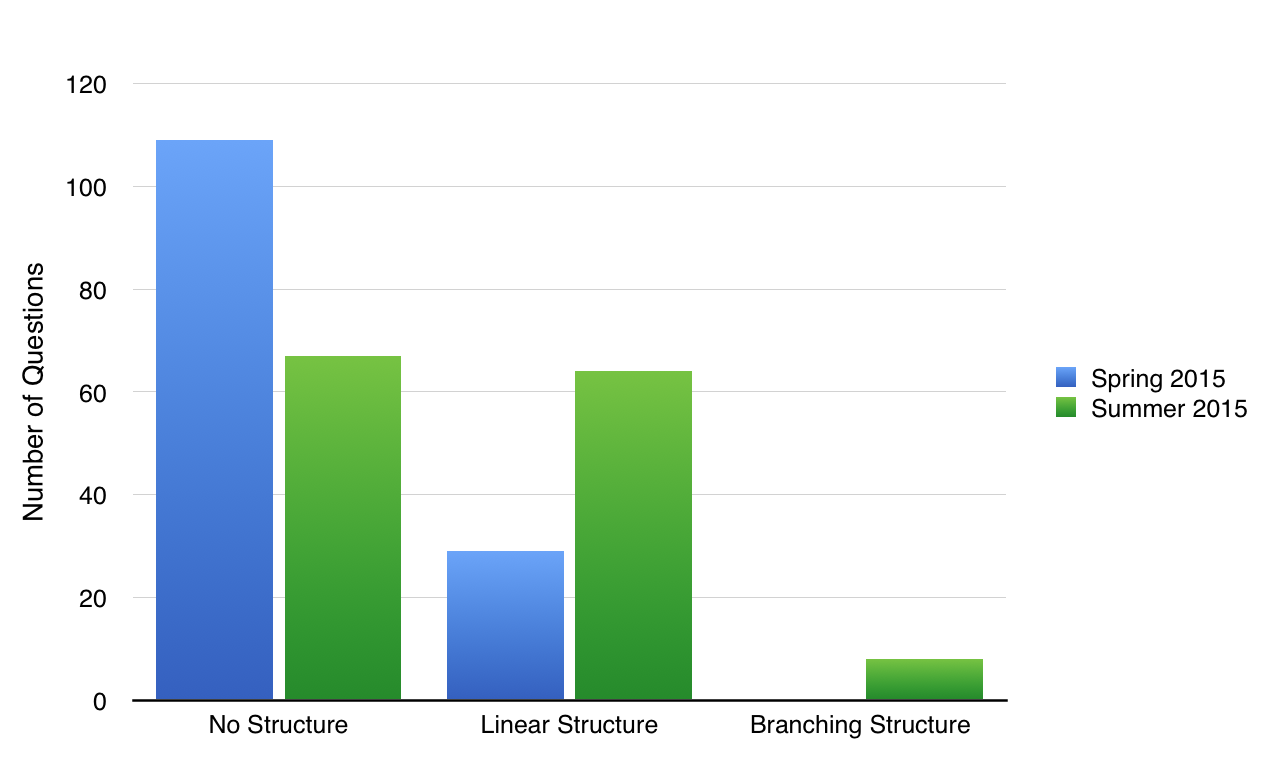
\includegraphics[width=6in]{img/chapter4/question_statistics}
	\caption[The Number of Linear and Branching Questions Implemented in the PHYS 24100 Homework]{The Number of Linear and Branching Questions Implemented in the PHYS 24100 Homework}
  \label{fig:questionStatistics}
\end{figure}


\subsection{Postscripts}

At the end of each problem, we present one or two qualitative questions that expand on the topics covered in the preceding question. For example, after solving a circuit question, we might ask students how the problem would change if the battery was connected in reverse. These postscript questions are not counted for a grade; instead, they are meant to encourage deeper thought about the problem. This deeper thought about the homework question is meant to expand student’s knowledge of the concepts at hand.

Oftentimes, we will use this section to ask slightly more obscure questions that would not usually be fitting for a graded homework. For example, we might ask the introductory physics students to speculate how Maxwell's equations would change if magnetic monopoles did exist. Or we might ask the students to estimate the electric potential energy needed to launch a projectile to the moon. Once again, these questions are not meant to be harshly graded - only to make the students play around with the concepts at hand.

\section{Analysis Tools}

\subsection{CHIP}

\gls{chip} has a useful set of built in statistical analysis tools. Most of the quantiative analysis that we plan to do will take place through the \gls{chip} \gls{gui}. However, \gls{chip} does not support operations like Student T-Tests or ANOVA. These additional operations will be done using R or an equivalent statistical analysis program.

\subsection{Muffin}

Over the course of this project, we will have to deal with data from a variety of sources. For example, we will have to review CSV data from the \gls{chip} website, JSON data from the Piazza website, audio data from focus group transcripts, and written data from notes taken by teaching assistants over the course of the study. We need a simple and efficient way to translate one data format into another so that it can be used with PHYS 24100.

I have written an open-source data analysis toolbox called Muffin that will handle this information. Muffin is a set of Ruby functions that will simply read and write data to a format appropriate for our study. The source code for Muffin is hosted on \index{Ruby Gems}Ruby Gems as well as on my personal \index{GitHub}GitHub page.

Muffin is simply a toolbox that converts data from one format to another. It does not store anything or conduct analysis in any way. Thus, privacy is maintained, even when the Muffin source code is freely distributed online.

\section{Current Results}

\section{BEMA Results}

We use the \gls{bema} exam to conduct a preliminary analysis of the effectiveness of the \gls{cita} on \gls{chip} system. In \ref{fig:bemaSp15} I plot the pre- and post-test scores of students taking the exam in the spring 2015 semester. These students are in the on-campus, PHYS 24100 course. In \ref{fig:bemaSu15} I plot the pre- and post-test scores of students taking the exam in the summer 2015 semester.

\begin{figure}[!htb]
	\centering
	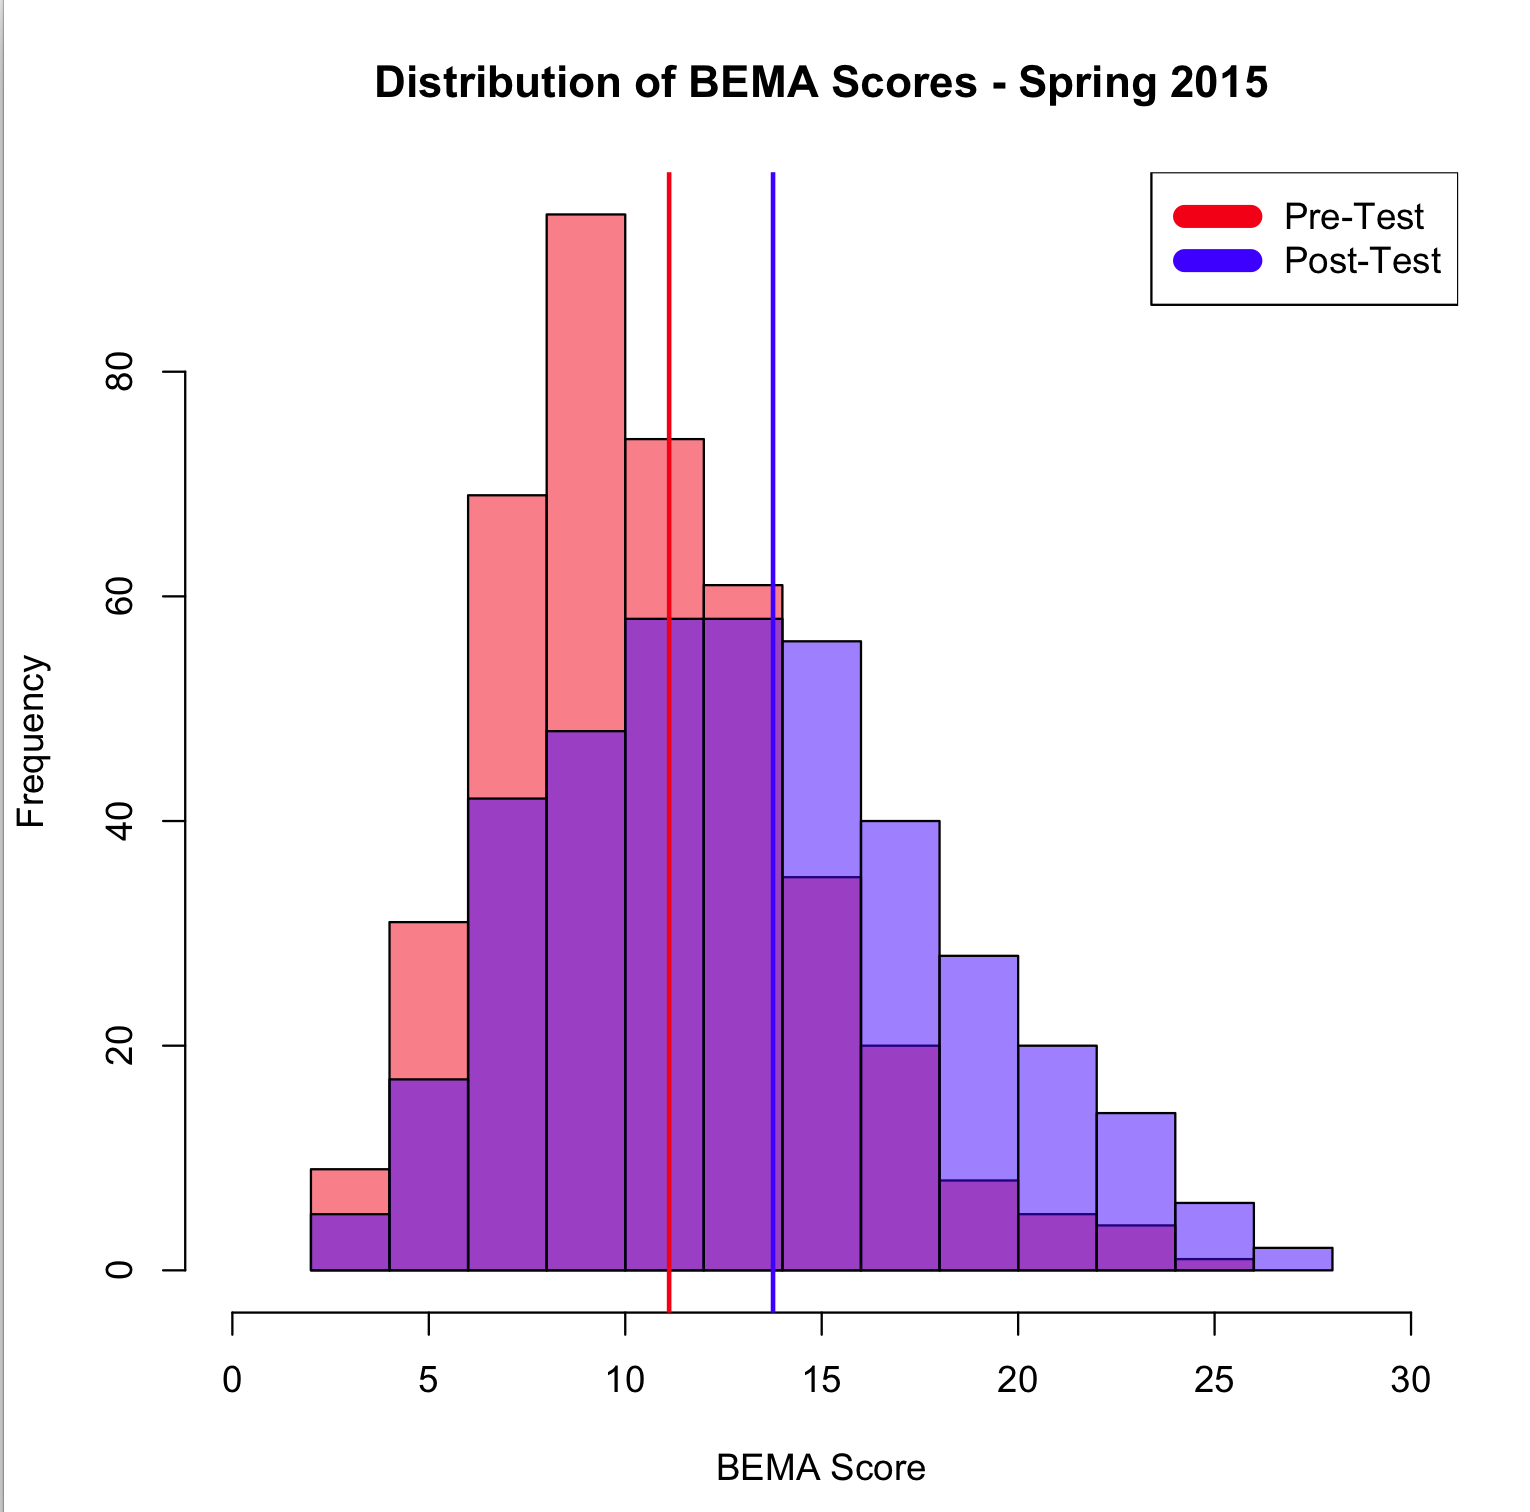
\includegraphics[width=6in]{img/chapter4/bema_spring_2015}
	\caption[BEMA Scores for the Spring 2015 PHYS 24100 Class]{BEMA Scores for the Spring 2015 PHYS 24100 Class}
  \label{fig:bemaSp15}
\end{figure}

\pagebreak

\begin{landscape}
\begin{table}[!ht]
  \centering
  \begin{tabular}{|l|l|l|}
    \hline
    \textbf{Statistic} & \textbf{Value} & \textbf{Interpretation}\\
	\hline
	Mean of Pre-Test & 11.117 & \\
	\hline
	Mean of Post-Test & 13.761 & \\
	\hline
	Standard Deviation of Pre-Test & 3.923 & \\
	\hline
	Standard Deviation of Post-Test & 5.030 & \\
	\hline
	Shapiro-Wilk Normality Test of Pre-Test & p-value = 9.24e-08 & The sample is not normally distributed \\
	\hline
	Shapiro-Wilk Normality Test of Post-Test & p-value = 0.000138 & The sample is not normally distributed \\
	\hline
	Wilcoxon Signed-Rank Test of Pre-Test and Post-Test & p-value = 9.74e-15 & The difference between the means is statistically significant. \\
	\hline
	Cohen's D of Pre-Test and Post-Test & 0.588 & ``Medium'' effect size \\
	\hline
  \end{tabular}
  \caption{Spring 2015 BEMA Statistics}
  \label{tab:statsSp15}
\end{table}
\end{landscape}

\begin{figure}[!htb]
	\centering
	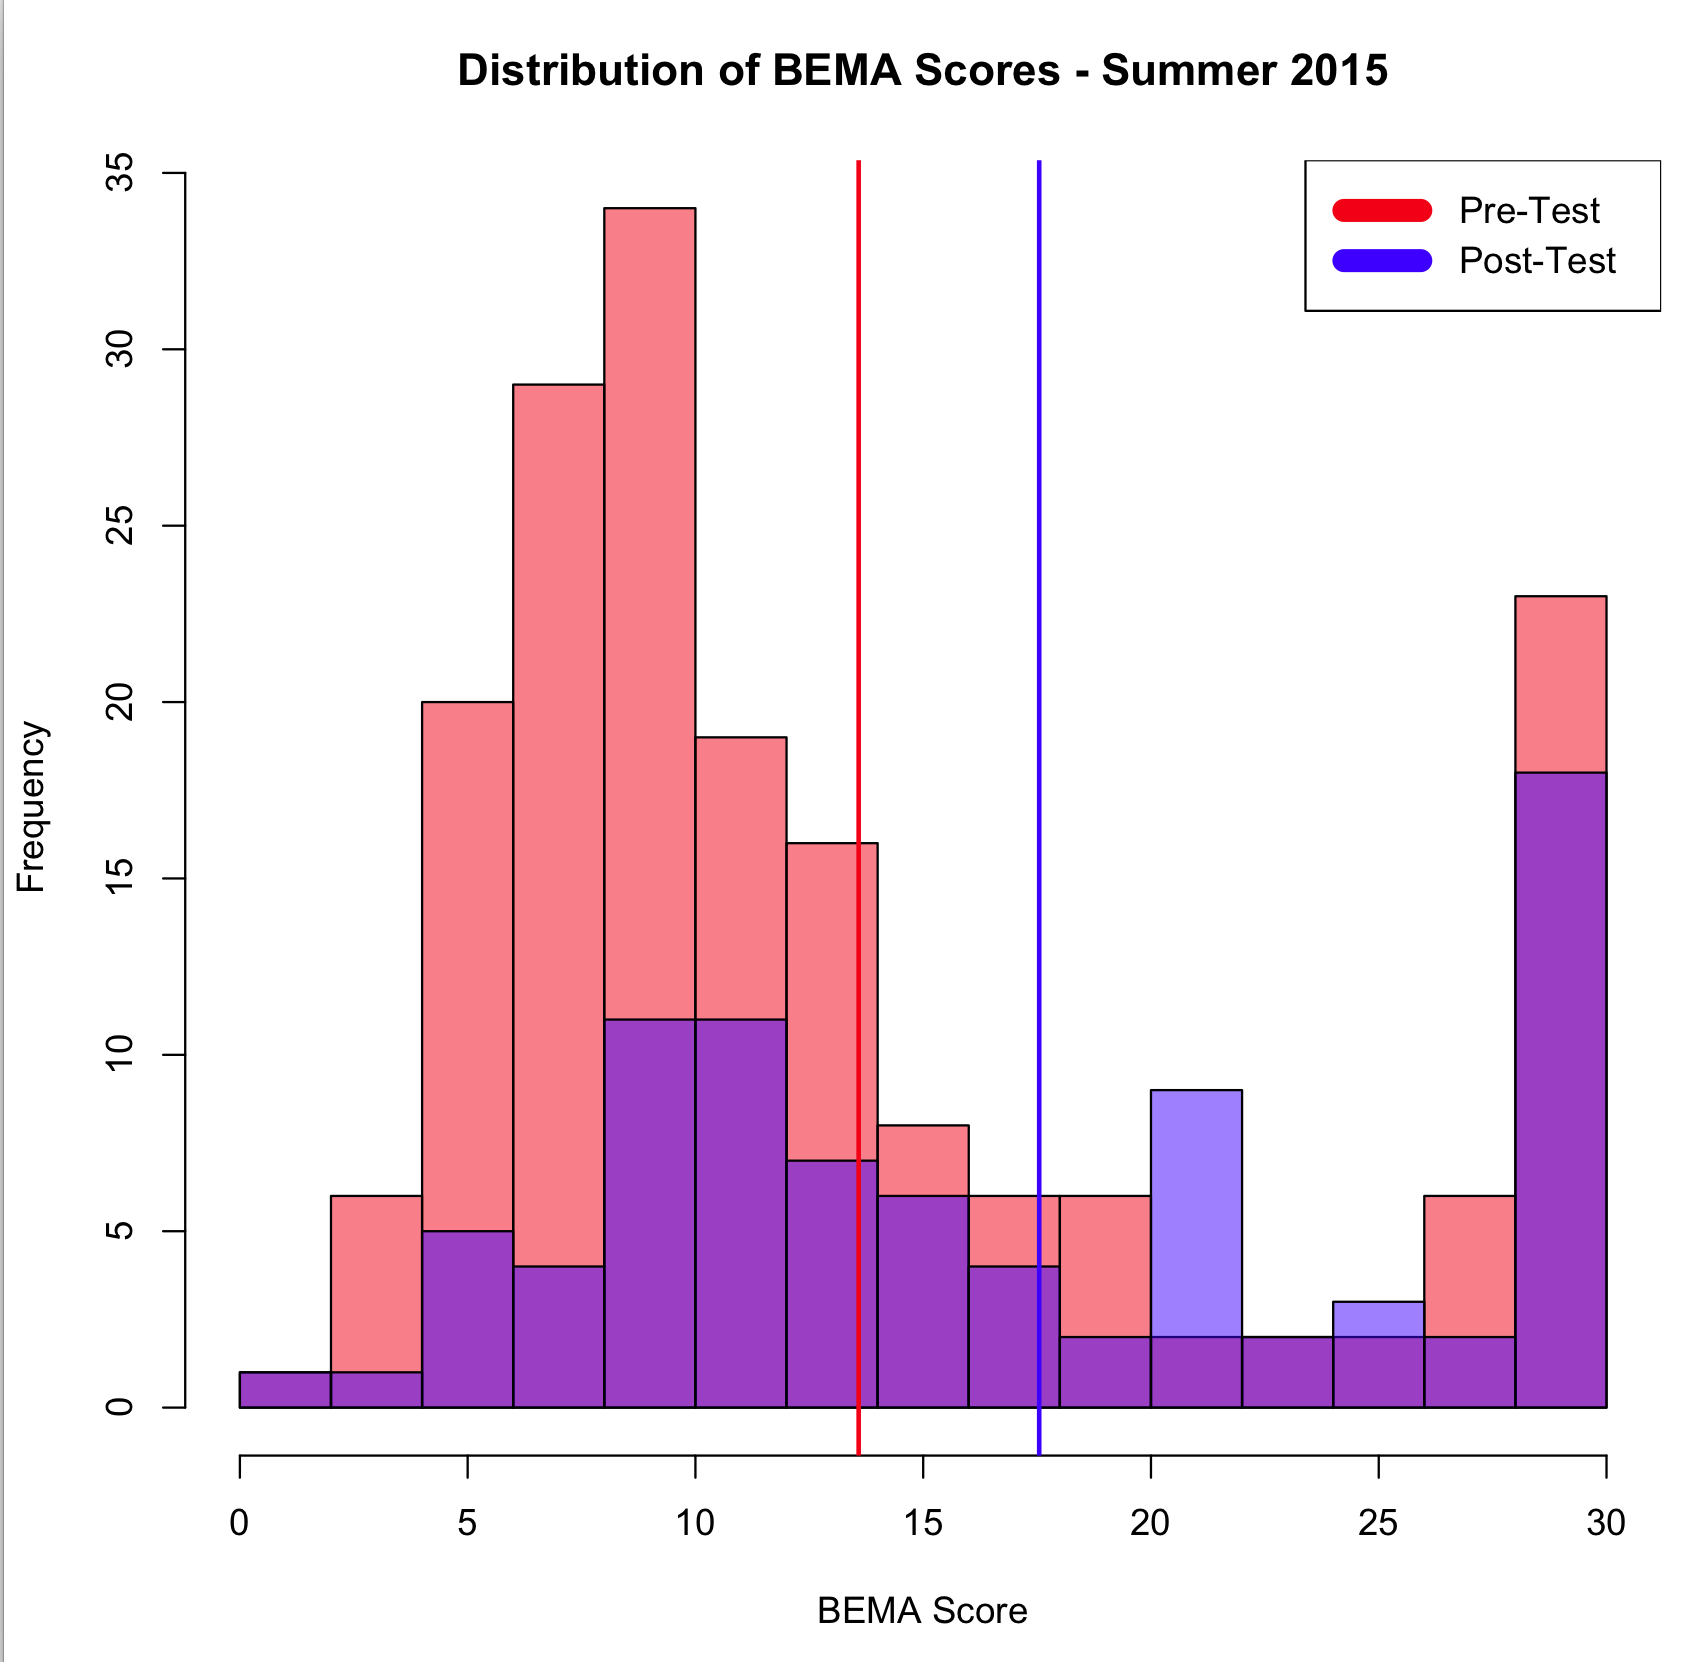
\includegraphics[width=6in]{img/chapter4/bema_summer_2015}
	\caption[BEMA Scores for the Summer 2015 PHYS 24100 Class]{BEMA Scores for the Summer 2015 PHYS 24100 Class}
  \label{fig:bemaSu15}
\end{figure}

\pagebreak

\begin{landscape}
\begin{table}[!ht]
  \centering
  \begin{tabular}{|l|l|l|}
    \hline
    \textbf{Statistic} & \textbf{Value} & \textbf{Interpretation}\\
	\hline
	Mean of Pre-Test & 13.583 & \\
	\hline
	Mean of Post-Test & 17.547 & \\
	\hline
	Standard Deviation of Pre-Test & 8.169 & \\
	\hline
	Standard Deviation of Post-Test & 8.500 & \\
	\hline
	Shapiro-Wilk Normality Test of Pre-Test & p-value = 1.599e-12 & The sample is not normally distributed \\
	\hline
	Shapiro-Wilk Normality Test of Post-Test & p-value = 1.332e-05 & The sample is not normally distributed \\
	\hline
	Wilcoxon Signed-Rank Test of Pre-Test and Post-Test & p-value = 4.916e-05 & The difference between the means is statistically significant. \\
	\hline
	Cohen's D of Pre-Test and Post-Test & 0.479 & ``Medium'' effect size \\
	\hline
  \end{tabular}
  \caption{Summer 2015 BEMA Raw Statistics}
  \label{tab:statsSu15}
\end{table}
\end{landscape}

The best way to compare the scores between the two classes is to compare the average gains of students rather than the \gls{bema} averages themselves. The Hake factor is calculated using the following formula:

\begin{equation}
	g = \frac{Post - Pre}{31 - Pre}
\end{equation}

Note that the 31 in the denominator comes from the fact that the maximum score on the \gls{bema} exam is 31 points. In \ref{fig:hakeFull} I plot the Hake factors for the two semesters. In the plots, I eliminate one outlier from the summer 2015 course that had a Hake factor of -22.

\begin{figure}[!htb]
	\centering
	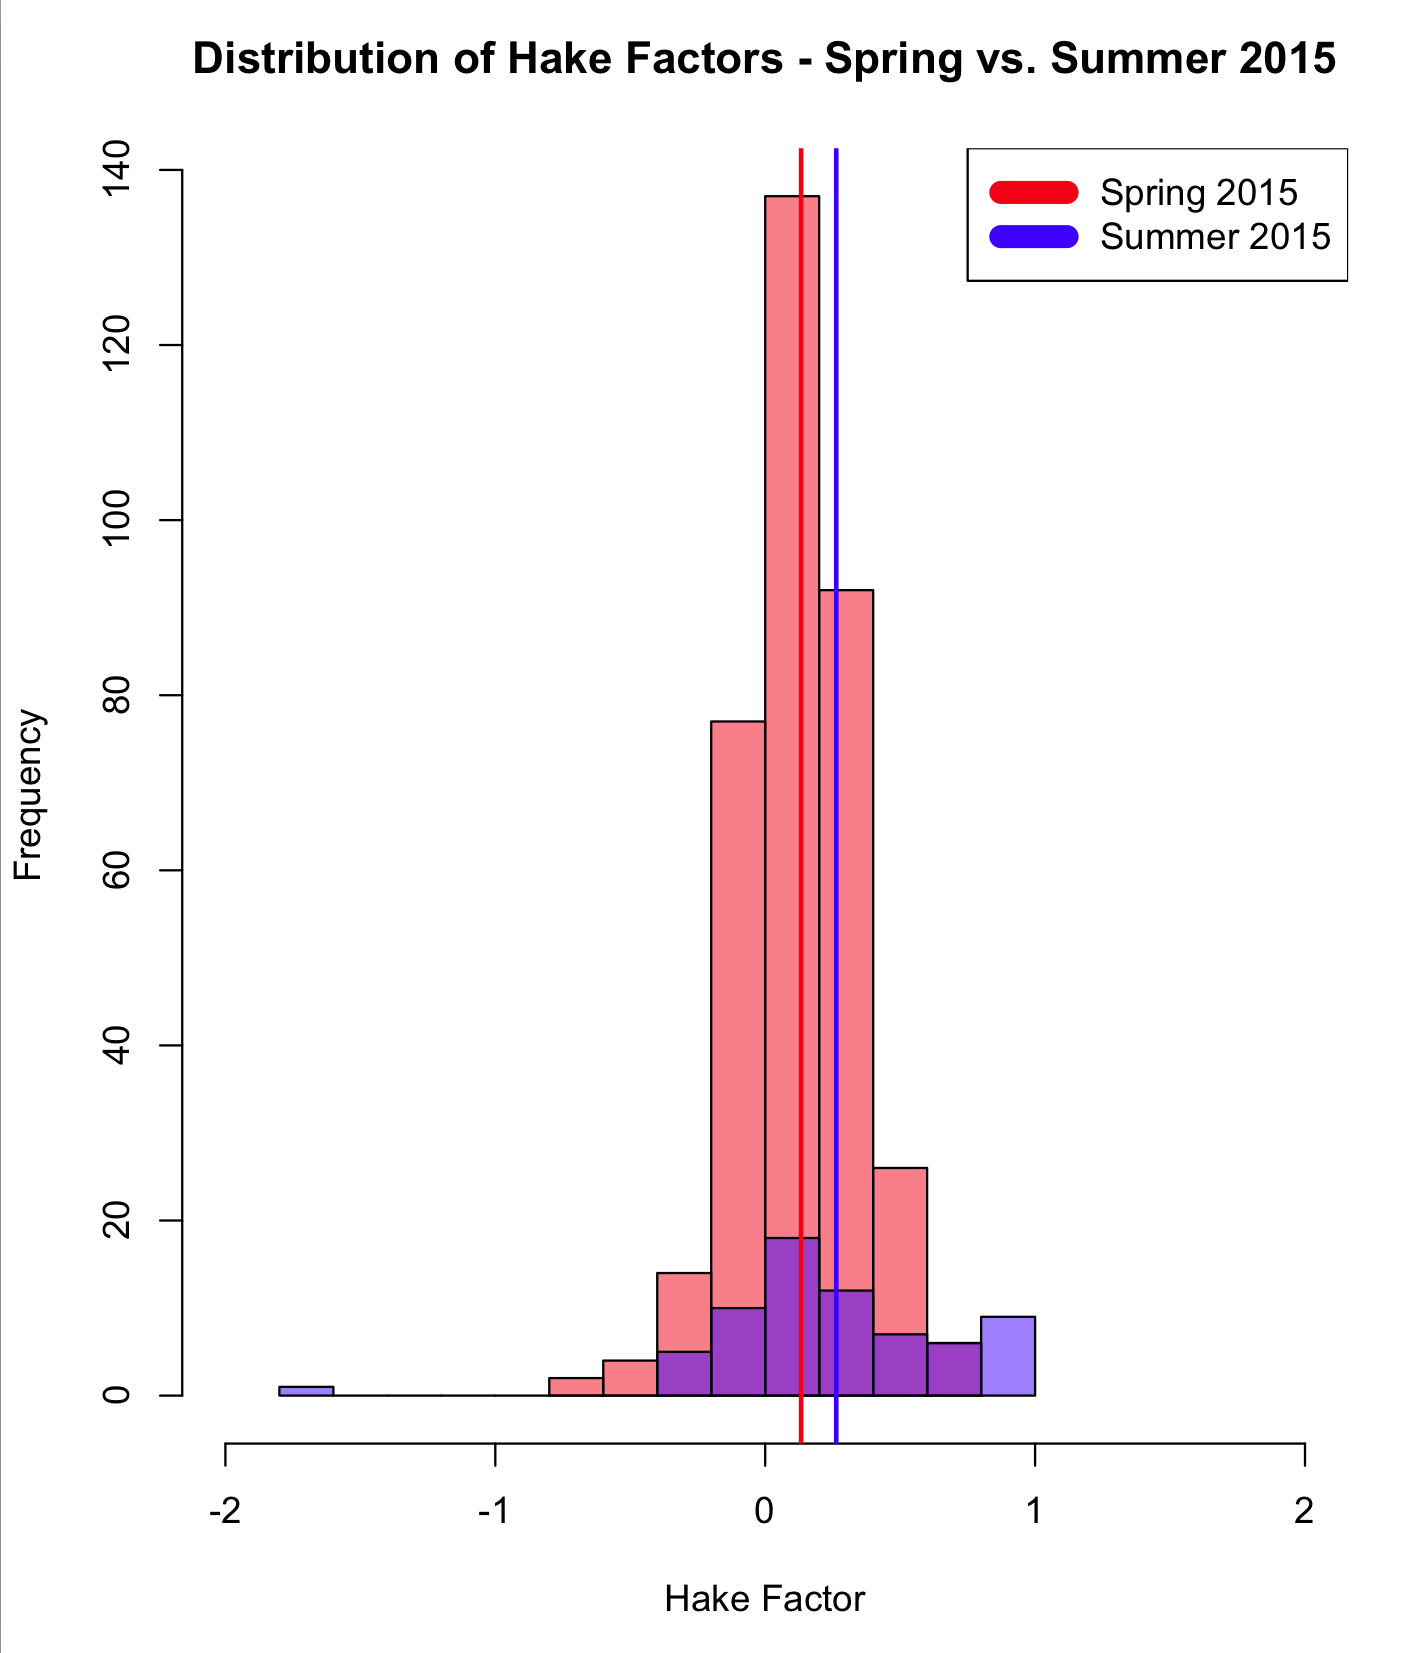
\includegraphics[width=6in]{img/chapter4/hake_spring_vs_summer_full}
	\caption[Comparison of Hake Factors on the BEMA Between Spring and Summer 2015]{Comparison of Hake Factors on the BEMA Between Spring and Summer 2015}
  \label{fig:hakeFull}
\end{figure}

During the summer, we noticed a lot of scores that seemed very inflated. We suspect that many students were cheating on the \gls{bema} exam since they could take it online without any supervision. This was not a problem for the spring 2015 PHYS 24100 class because they all took the exam under closely monitored conditions. Thus, in order to better compare the Hake factors, I eliminte all data points from the summer where a student's pre-test score was 27 or higher. The new plot is shown in \ref{fig:hakeFiltered}.

\begin{figure}[!htb]
	\centering
	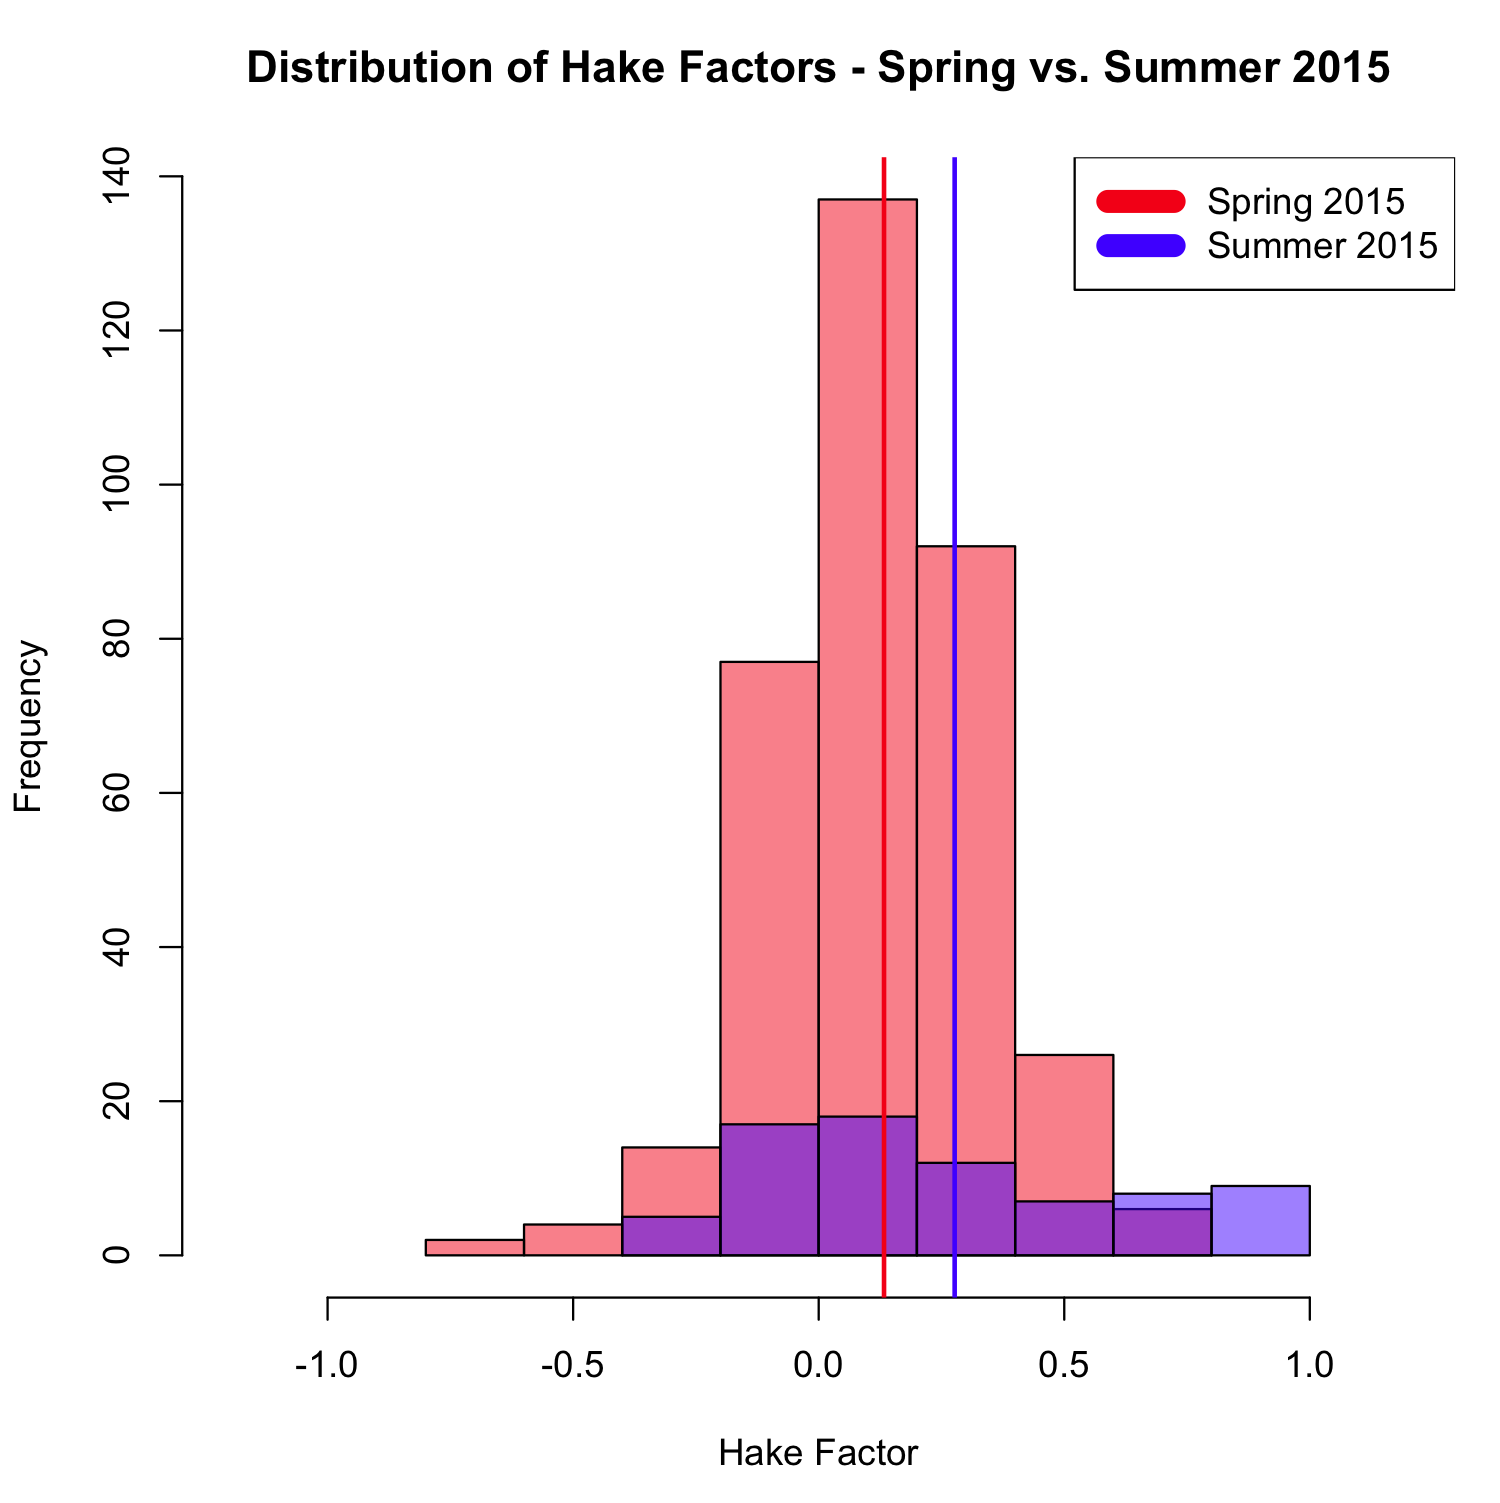
\includegraphics[width=6in]{img/chapter4/hake_spring_vs_summer_filtered}
	\caption[Comparison of Hake Factors on the BEMA Between Spring and Summer 2015, Filtered to Eliminate Outliers and Pre-Test Grades Over 26/31 Points ]{Comparison of Hake Factors on the BEMA Between Spring and Summer 2015, Filtered to Eliminate Outliers and Pre-Test Grades Over 26/31 Points}
  \label{fig:hakeFiltered}
\end{figure}

\begin{landscape}
\begin{table}[!ht]
  \centering
  \begin{tabular}{|l|l|l|}
    \hline
    \textbf{Statistic} & \textbf{Value} & \textbf{Interpretation}\\
	\hline
	Mean of Spring Hake Factors & 0.133 & \\
	\hline
	Mean of Summer Hake Factors & 0.263 & \\
	\hline
	Standard Deviation of Spring Hake Factors & 0.208 & \\
	\hline
	Standard Deviation of Summer Hake Factors & 0.440 & \\
	\hline
	Shapiro-Wilk Normality Test of Spring Hake Factors & p-value = 6.683e-05 & The sample is not normally distributed \\
	\hline
	Shapiro-Wilk Normality Test of Summer Hake Factors & p-value = 8.509e-06 & The sample is not normally distributed \\
	\hline
	Wilcoxon Signed-Rank Test of Hake Factors & p-value = 0.009334 & The difference between the means is statistically significant. \\
	\hline
	Cohen's D of Hake Facrors & 0.503 & ``Medium'' effect size \\
	\hline
  \end{tabular}
  \caption{Spring vs. Summer 2015 Hake Factors, filtering out any data with a pre-test score above 26/31.}
  \label{tab:compareSpSu15}
\end{table}
\end{landscape}

\begin{figure}[!htb]
	\centering
	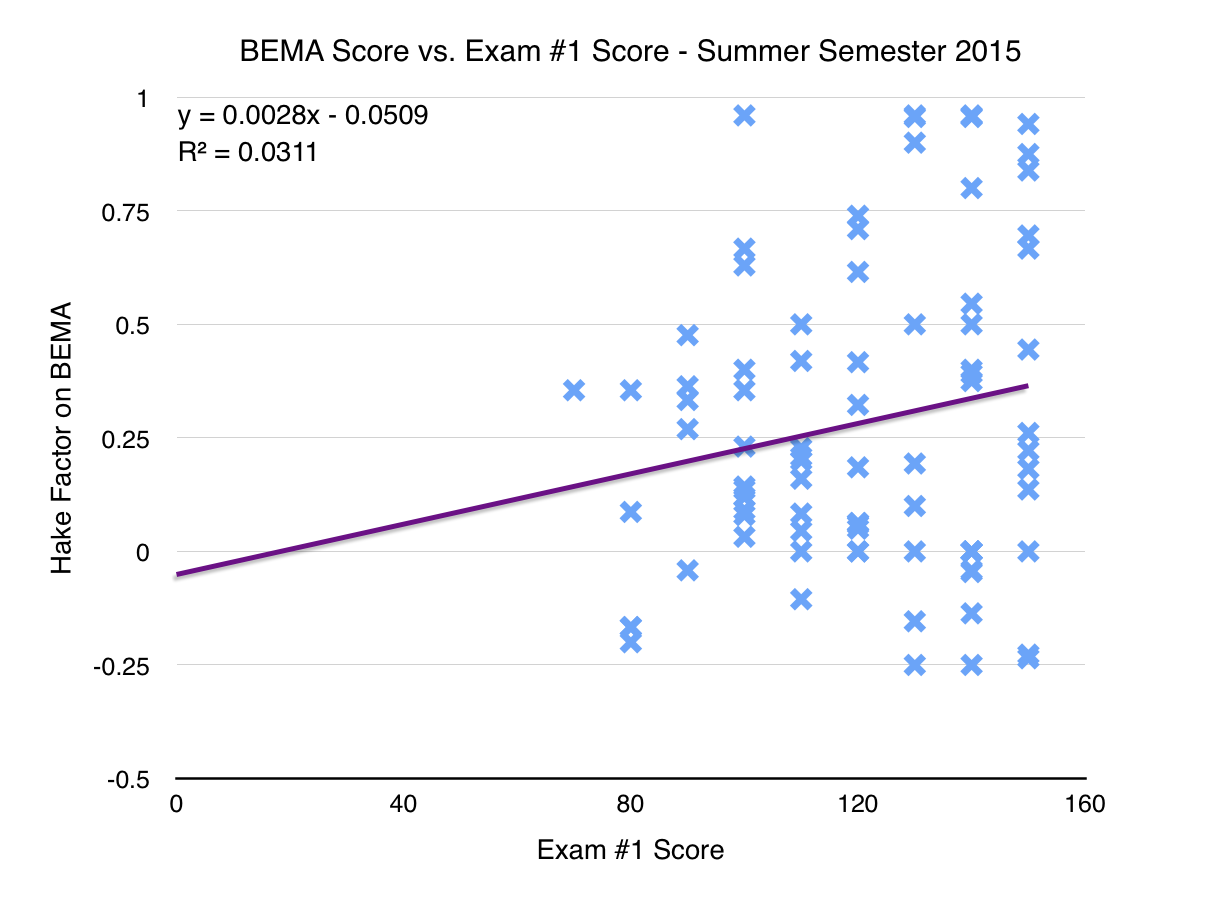
\includegraphics[width=6in]{img/chapter4/bema_vs_ex1_su15}
	\caption[BEMA Hake Factor vs. Exam \#1 Scores]{BEMA Hake Factor vs. Exam \#1 Scores}
  \label{fig:bemaVsExOneSu15}
\end{figure}

\begin{figure}[!htb]
	\centering
	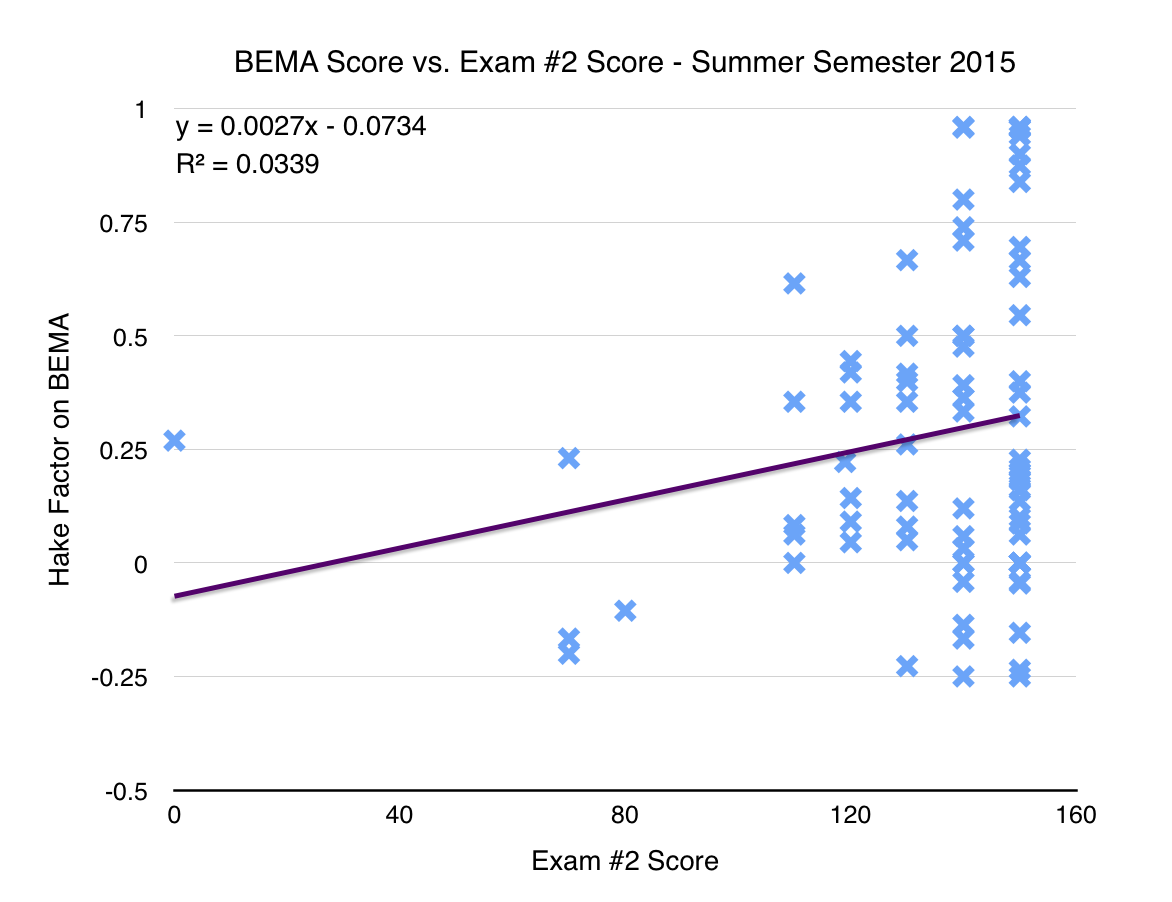
\includegraphics[width=6in]{img/chapter4/bema_vs_ex2_su15}
	\caption[BEMA Hake Factor vs. Exam \#2 Scores]{BEMA Hake Factor vs. Exam \#2 Scores}
  \label{fig:bemaVsExTwoSu15}
\end{figure}

\begin{figure}[!htb]
	\centering
	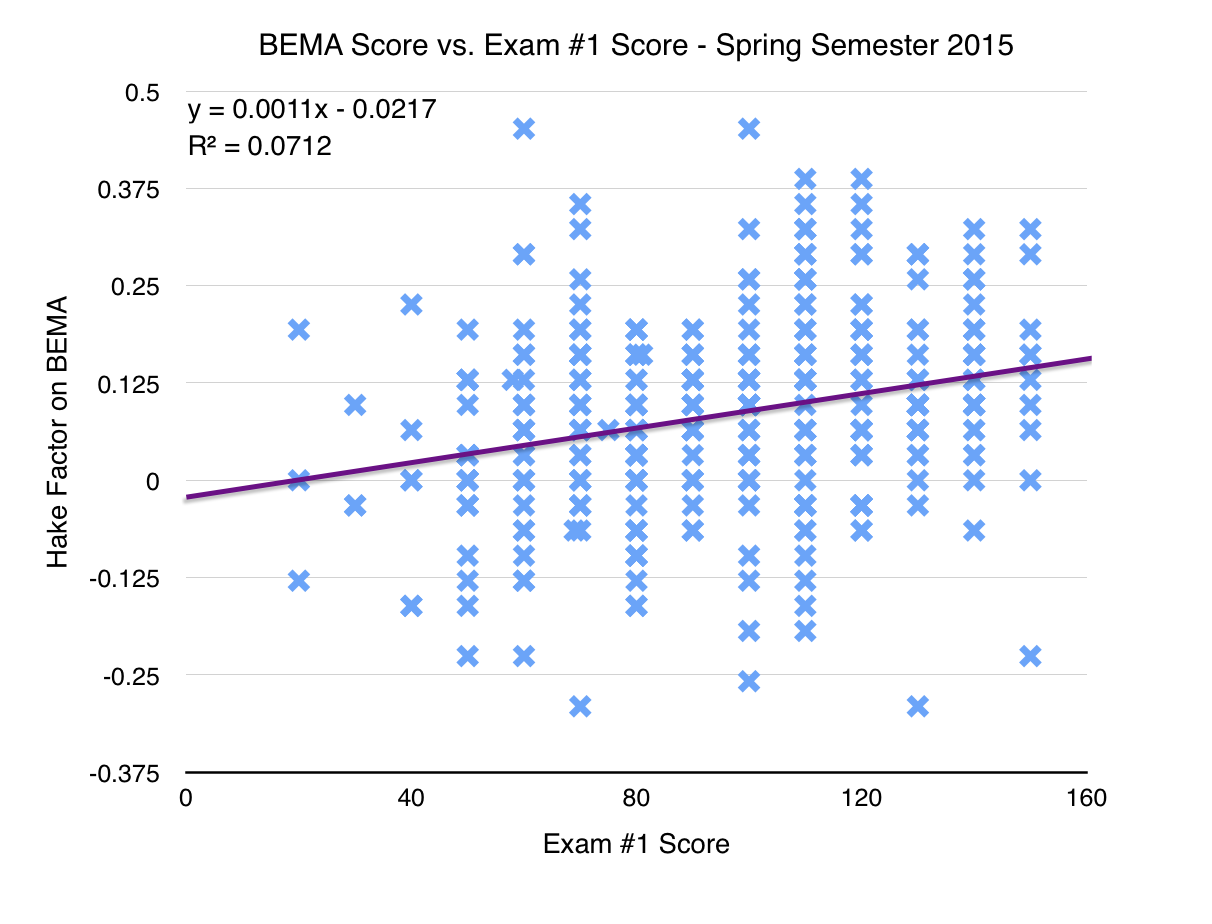
\includegraphics[width=6in]{img/chapter4/bema_vs_ex1_sp15}
	\caption[BEMA Hake Factor vs. Exam \#1 Scores]{BEMA Hake Factor vs. Exam \#1 Scores}
  \label{fig:bemaVsExOneSp15}
\end{figure}

\begin{figure}[!htb]
	\centering
	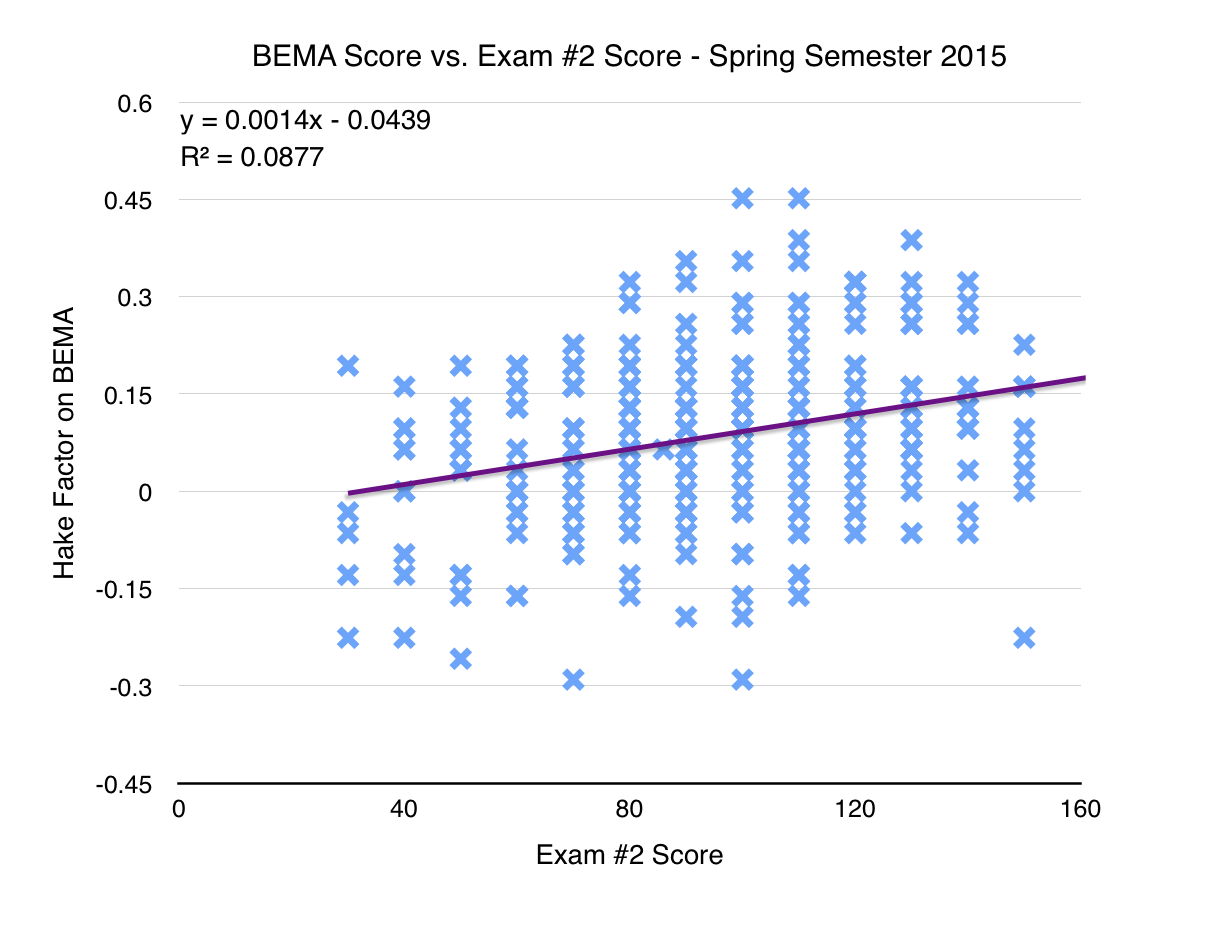
\includegraphics[width=6in]{img/chapter4/bema_vs_ex2_sp15}
	\caption[BEMA Hake Factor vs. Exam \#2 Scores]{BEMA Hake Factor vs. Exam \#2 Scores}
  \label{fig:bemaVsExTwoSp15}
\end{figure}

On first glance, the summer 2015 semester outperformed the spring 2015 semester. Although the initial results for the \gls{bema} look promising, we do need to put them in context. First, the spring and summer sections of PHYS 24100 are two very different classes with two very different student bodies. The spring semester is a more traditional student body while the summer semester has the advantage of the internet as a reference (all of the students were online during the summer 2015 semester).

\subsection{Conclusions}

First and foremost, we need to ensure that student performance does not suffer because of our system. Due to the gains in score data from above, we are assured that student performance is postively, not negatively affected by the \gls{cita} system.

\subsection{Future Work}

We plan to conduct our first focus group sessions and student interviews in the fall 2015 semester. Thus, as of now there is no focus group data that can be analyzed. Additionally, we plan to administer and grade the multi-step problem to on-campus sections of PHYS 24100 starting in the fall 2015 semester. Again, this analysis will be started in the upcoming months. Both of these branches of analysis are dependent on IRB approval from Purdue University.

The summer 2015 semester of PHYS 24100 will take their final exams during the week of my preliminary presentation. Thus, the analysis of their exit survey data, end-of-the-semester feedback, final exam data, and final grade data will be deferred to the fall 2015 semester.


-> Purposeful Sampling
-> Cite von glosserfeld - add foundational work to report.
